\documentclass[output=paper]{langscibook}
\ChapterDOI{10.5281/zenodo.6977052}

\author{Gloria Corpas Pastor\orcid{}\affiliation{University of Malaga} and Fernando Sánchez Rodas\orcid{}\affiliation{University of Malaga}}

\title[NLP-enhanced shift analysis of named entities]{NLP-enhanced shift analysis of named entities in an English<>Spanish intermodal corpus of European petitions}

\abstract{This chapter aims at presenting an NLP-enhanced corpus-based analysis of the translation and interpreting shifts observed in the named entities (NEs) of PETIMOD, an English<>Spanish intermodal corpus of written and oral mediated texts from the Committee on Petitions of the European Parliament. Our main assumption is that shifts in institutional genres mostly occur in the transfer of NEs, and that NLP techniques such as automatic Named Entity Recognition (NER) can be applied to systematically extract and compare examples of these shifts, leading to the (possible) verification of translational and/or interpretational constraints. Results show that traits like normalisation, transformation and simplification depend not only on the language direction or the mediation mode, but also on the semantic category (person, organisation, etc.) of the NE involved. Further studies are needed in order to correlate observed shifts with different NE taxonomies.}

\IfFileExists{../localcommands.tex}{
  \addbibresource{../localbibliography.bib}
  % add all extra packages you need to load to this file

\usepackage{tabularx,multicol}
\usepackage{url}
\urlstyle{same}

\usepackage{listings}
\lstset{basicstyle=\ttfamily,tabsize=2,breaklines=true}

\usepackage{langsci-basic}
\usepackage{langsci-optional}
\usepackage{langsci-lgr}
\usepackage{langsci-osl}
% \usepackage{./langsci/styles/langsci-lgr}
% \usepackage{./langsci/styles/langsci-osl}
% \usepackage{langsci-gb4e}

\usepackage{tikz}
\usetikzlibrary{patterns,calc}
\pgfdeclarepatternformonly{south east lines}{\pgfqpoint{-0pt}{-0pt}}{\pgfqpoint{3pt}{3pt}}{\pgfqpoint{3pt}{3pt}}{
    \pgfsetlinewidth{0.6pt}
    \pgfpathmoveto{\pgfqpoint{0pt}{3pt}}
    \pgfpathlineto{\pgfqpoint{3pt}{0pt}}
    \pgfpathmoveto{\pgfqpoint{.2pt}{-.2pt}}
    \pgfpathlineto{\pgfqpoint{-.2pt}{.2pt}}
    \pgfpathmoveto{\pgfqpoint{3.2pt}{2.8pt}}
    \pgfpathlineto{\pgfqpoint{2.8pt}{3.2pt}}
    \pgfusepath{stroke}}
    
\usepackage{stmaryrd}
\usepackage{wasysym}
\usepackage{multirow}
\usepackage{caption}
\usepackage{subcaption}
\usepackage{mathrsfs}
\usepackage{qtree}

\usepackage{linguex}


  %pminos do not split footnotes
% \interfootnotelinepenalty=10000 %Footnote in Laporte chapters has to be split SN


%\DeclareIndexNameFormat{default}{%
%\nameparts{#1}%
%\usebibmacro{index:name}%
%{\index[names]}%
%{\namepartfamily}%
%{\namepartgiveni}%
% {}% L1
% {}% L2
%{\namepartprefix}% generates spurious space L3
%{\namepartsuffix}% generates spurious space L4
%}

%  {\DeclareIndexNameFormat{default}{%
%     \usebibmacro{index:name}{\index[names]}{#1}{#3}{#5}{#7}}}

%\DeclareIndexNameFormat{default}{%
%  \usebibmacro{index:name}{\sindex[nom]}{#1}{#3}{#5}{#7}}

%\DeclareIndexNameFormat{default}{%
%  \usebibmacro{index:name}{\sindex[person]}{#1}{#3}{#5}{#7}}
%\DeclareIndexNameFormat{default}{%
%\nameparts{#1} \usebibmacro{index:name}{\sindex[person]]}{\namepartfamily}{‌​\namepartgiven}{\nam‌​epartprefix}{\namepa‌​rtsuffix}}

%\newcommand{\smiley}{:)}

%\renewbibmacro*{index:name}[5]{%
%\usebibmacro{index:entry}{#1}%
%{\iffieldundef{usera}{}{\thefield{usera}\actualoperator}\mkbibindexname{#2}{#3}{#4}{#5}}}

% \newcommand{\noop}[1]{}

%remove for final
%\overfullrule=1mm

\newcommand{\tobi}[2]}}
\renewcommand{\S}[1]{\tobi{#1}{\textsc{*}}}

% this volume references
% puts: [this volume]
% already defined: \citetv
%\newcommand{\citepv}[1]{(\citeauthor{#1} \citeyear*{#1} [this volume])}
\newcommand{\citealtv}[1]{\citeauthor{#1} \citeyear*{#1} [this volume]}

%parentheses around example number
\newcommand{\pref}[1]{(\ref{#1})}

% in-text examples

\newcommand{\lnex}[1]{\textit{#1}} %target lang word
\newcommand{\lnlit}[1]{(lit.: `#1')} %literal reading
\newcommand{\lnlat}[1]{(#1)} % latinization
\newcommand{\lntrans}[1]{`#1'} %translation
\newcommand{\lnexl}[2]%
{\lnex{#1}{} \lnlat{#2}} % ex with latinization
\newcommand{\lnexlat}[3]{\lnex{#1}{} \lnlat{#2}{} \lntrans{#3}} % ex with latinization and tranl.

%ch01
\newcommand{\co}[1]{\mbox{\textbf{#1}}}

%ch09

\newcommand{\cyrbulg}[1]{\begin{otherlanguage*}{bulgarian}#1\end{otherlanguage*}}


%ch10
\newcommand{\nlp}{{\small NLP}}
\newcommand{\mwe}{{\small MWE}}
\newcommand{\rae}{{\small RAE}}
\newcommand{\lvc}{{\small LVC}}
\newcommand{\pos}{{\small P}o{\small S}}
%\newcommand{\todo}[1]{ \textcolor{red}{#1} }

%\renewcommand{\labelenumi}{\theenumi}
%\ainamefmt{{vv}{ll}{, ff}{, jj}} % fullname

\newcommand{\biberror}[1]{{\color{red}#1}}

\newcommand{\osenovaitem}{--~}
  %% hyphenation points for line breaks
%% Normally, automatic hyphenation in LaTeX is very good
%% If a word is mis-hyphenated, add it to this file
%%
%% add information to TeX file before \begin{document} with:
%% %% hyphenation points for line breaks
%% Normally, automatic hyphenation in LaTeX is very good
%% If a word is mis-hyphenated, add it to this file
%%
%% add information to TeX file before \begin{document} with:
%% %% hyphenation points for line breaks
%% Normally, automatic hyphenation in LaTeX is very good
%% If a word is mis-hyphenated, add it to this file
%%
%% add information to TeX file before \begin{document} with:
%% \include{localhyphenation}
\hyphenation{
    Beck-man
    Ngu-yen
    back-chan-nel
    back-chan-nels
    mo-not-o-nous
    ste-reo-typ-i-cal
}

\hyphenation{
    Beck-man
    Ngu-yen
    back-chan-nel
    back-chan-nels
    mo-not-o-nous
    ste-reo-typ-i-cal
}

\hyphenation{
    Beck-man
    Ngu-yen
    back-chan-nel
    back-chan-nels
    mo-not-o-nous
    ste-reo-typ-i-cal
}

  \togglepaper[8]%%chapternumber
}{}

\begin{document}
\maketitle
%\shorttitlerunninghead{}%%use this for an abridged title in the page headers






\section{Introduction}\label{sec:corpas:1}

To the present day, a considerable amount of corpus-based research in translation and interpreting has relied on the European Parliament (EP) as a main or only source. Among the European Union (EU) institutions, the Parliament provides an open access repository of both official documents and speeches in a wide range of languages and topics. Before the appearance of intermodal corpora such as EPTIC \citep{BernardiniEtAl2016}, the EP had already been used as a source for building translation corpora, e.g., Europarl  \citep{Koehn2005}, the European Parliamentary Comparable and Parallel Corpora, or ECPC (\citealt{MartinezSerrat2012}), and the EU resources at Sketch Engine \citep{BaisaEtAl2016}. In the field of corpus-based interpreting studies, it was early pointed out that EP linguistic material could provide researchers with numerous advantages \citep{Bendazzoli2010}. The European Parliament Interpreting Corpus (EPIC) is an example of this \citep{RussoEtAl2012}. However, researchers have not yet attended the call. In spite of their unquestionable relevance and high-level complexity, legislative chambers have not received that much attention from linguistics until very recently \citep{calzada-perez_researching_2017}.\footnote{See \citet{Veroz2014a, Veroz2014b, Veroz2017} and \citet{PrietoRamos2019} for examples of corpus-based discursive and/or linguistic analysis in this field.} Bibliometric analyses of Europarl (one of the largest multilingual corpora available) show that it has hardly been used in translation studies \citep{Ustaszewski2019}.\footnote{In order to make the wealth of linguistic data easily and readily available to the translation studies community, a toolkit named EuroparlExtract has been recently developed \citep{Ustaszewski2019}.} Reasons for this little academic interest may include corpora distribution in a format that largely disregards the needs of translation research and practice (ibid.) and the need for unexplored, more down-to-earth studies which empirically look at the compared properties of source texts, translations and interpretations and offer a modern, technology-based twist on the methodologies involved.

Against this background, we hypothesise that texts and speeches which originated in the Committee on Petitions of the European Parliament provide an excellent source for the observation of shifts in institutional translation and interpreting, and that shifts in these genres are mostly given in the transfer of Named Entities (NEs). We also assume that recent techniques based on Natural Language Processing (NLP) can be applied to the recognition, extraction and comparison of segments with NEs in two languages and/or modes, as a systematic way of observing shifts between them and proving (or not) the existence of translation and interpreting universals in the analysed texts. To this end, our main research objectives are as follows: 

\begin{itemize}
\item 
compile an intermodal, bidirectional corpus (English<>Spanish) of translations and interpretations (plus their different, corresponding source texts) of suitable genres from the EP Committee on Petitions;
\item 
apply NLP-based techniques (Named Entity Recognition) on the said corpus in order to extract relevant units for the study of shifts in both languages and modes;
\item 
compare qualitatively and quantitatively the observed shifts in the English-Spanish translations and Spanish-English interpretations of the Committee;
\item 
draw conclusions on the relation of three different parameters (language, mode, and semantic category of the NEs) with the presence of translation and interpreting universal features in the analysed documents, especially of simplification traits.
\end{itemize}

In connection with the objectives above, the chapter presents the following structure. After this introduction (\sectref{sec:corpas:1}), \sectref{sec:corpas:2} covers basic notions related to communications in the Committee on Petitions. \sectref{sec:corpas:3} describes the PETIMOD corpus, with a special focus on data collection and design criteria. The NLP-based methodology deployed in this study is spelled out in \sectref{sec:corpas:4}; the main findings are presented in \sectref{sec:corpas:5} and then discussed in detail (\sectref{sec:corpas:6}). After considering some limitations of our study, \sectref{sec:corpas:7} offers some concluding remarks on the implications of intermodal corpora for research in translation and interpreting, with special reference to shifts, mediation types and functions, among other relevant issues.

\section{A brief overview of EU Petitions}\label{sec:corpas:2}

The right to petition is set out in the European legislation. Article 44 of the Charter of Fundamental Rights of the European Union ensures the right to petition to the European Parliament. And Article 227 of the Treaty on the Functioning of the European Union states that “any citizen of the Union, and any natural or legal person residing or having its registered office in a Member State” shall have the right to address a petition to the European Parliament \citep{EU2012}. A petition  may “take the form of a complaint, a request or an observation concerning problems related to the application of EU law or an appeal to the European Parliament to adopt a position on a specific matter” \citep{EP2020FAQ}.  After submission, original petitions are registered and given a number. Then, they are summarised (normally in English) and submitted to the members of the Committee on Petitions of the European Parliament for a decision on admissibility and follow-up (ibid.). This committee serves a core function within the governance of the Union, as it acts “as a bridge between Europeans and the EU institutions” \citep{EP2020PETI}.

As the Committee on Petitions plays an important, mediating role in the context of a multilingual institution and society such as the EU, translation and interpreting are especially relevant in assuring the transparency of its communications.  Petition summaries are translated and published in all official EU languages on the Petitions Portal of the European Parliament right after a decision on admissibility has been taken \citep{EP2020FAQ}.\footnote{In fact, petitions are one of the most frequent briefings for the translation trainees of the EP Schuman Traineeships (\url{https://ep-stages.gestmax.eu/website/homepage}).} The speeches of the committee meetings are also interpreted into each official language and published in the Webstreaming section of the European Parliament Committees website.\footnote{\url{https://www.europarl.europa.eu/committees/es/peti/meetings/webstreaming}.}  

As petitions are institutional texts, translators and interpreters have to deal with an important amount of terminology. As \citet[637--638]{Goffin1994} states, the language used in the EU texts, or eurolect, is no different in origin, semantic organization or morpho-syntactic characteristics from any other specialized dialect. Depending on the concept they represent,  EU terms are classified as \textit{euronymes,} i.e. terms coined for new institutional realities, or \textit{hétérolexies}, i.e. terms which convey notions and designations rooted in a given official EU language \citep[641]{Goffin1994}.\footnote{Examples of the two categories extracted from our named-entity recognition would be “Eurobarometer” (\textit{euronyme)} and “Boletín Oficial” (\textit{hétérolexie}).}

This classification indicates a prominence highly culture-bound of entities in this knowledge field. Entities are abstractions from external experience which are perceived as self-defined, that is, independent from each other in time and space (e.g. Dolors Montserrat, Bulgaria). Born out of quite specific worldly experiences, some entities pose a real challenge for translators and interpreters \citep{Mayoral1999}. This is especially true for institutional references, like the Spanish \textit{Civil Guard}, which are usually related to the political life of a society (\citealt{Martin1997}; \citealt{Ortega2002}). In the Committee on Petitions, where citizens and platforms strive to expose national problems and petitions are chosen by Members of the European Parliament (MEPs) on the basis of their political relevance, it is highly important to give these relevant entities a name (see \sectref{sec:corpas:4}).

\section{The PETIMOD Corpus}\label{sec:corpas:3}

The purpose of our compilation was to create an intermodal corpus of EU petitions suitable for the study of shifts in translated and interpreted NEs. The size of the corpus was initially limited to one month of institutional activity, and its medium written (see expanded size data in \sectref{sec:corpas:3.2}). The authorship of the documents was exclusively institutional and the topics were mostly agricultural and environmental, which was not determined by our sampling schema but given by the inherent frequency of the petitions. The publication date was a relevant criterion for the context of this research. As the elaboration of the paper ran parallel to the coronavirus crisis, a cancellation of the Committee activity and/or a change in the content of petitions was predicted. Therefore, the last Committee meeting before the health crisis (19\textsuperscript{th} and 20\textsuperscript{th} February 2020) was chosen as the main source of material.  Finally, the languages of the corpus were Spanish and English in their institutional or EU varieties (for a fully-fledged study on eurolects, see \citealt{Mori2018}).

\subsection{Data collection}\label{sec:corpas:3.1}

The retrieval, storing, and conversion of materials started with the oral transcriptions. First, the audiovisual material for the meeting was accessed via the Webstreaming section of the EP Committees site. Three sessions were available for this debate: two on 19 February 2020 (morning\footnote{\url{https://multimedia.europarl.europa.eu/es/peti-committee-meeting_20200219-0900-COMMITTEE-PETI_vd}.}  and afternoon\footnote{\url{https://multimedia.europarl.europa.eu/es/peti-committee-meeting_20200219-1430-COMMITTEE-PETI_vd}.}  sessions) and one on 20 February (morning\footnote{\url{https://multimedia.europarl.europa.eu/es/peti-committee-meeting_20200220-0930-COMMITTEE-PETI_vd}.}  session). We downloaded the complete recordings for both Spanish and English, obtaining six video files in high quality (HQ) .mp4 format.\footnote{Audio tracks are available for the original speeches and the interpretations into any official EU language, although only one version can be downloaded at once. Download is performed through a request system which allows for choosing between the complete session and a selected part, and also between different video qualities. After this, a download link is sent to the desired email account. Downloading high-quality videos was the less time-consuming option in the long term, since low and medium quality videos had to be re-downloaded because of visualization problems. This is a relevant point, as videos are quite helpful for identifying the speakers in each petition.} These were moved into a folder structure and coded with the date and time of each session plus the corresponding language abbreviation (e. g. “19feb1000\_EN.mp4”). The duration of each recording is indicated in \tabref{tab:corpas:1}.

\begin{table}
\begin{tabularx}{.8\textwidth}{Xr}

\lsptoprule

{\bfseries File(s) name(s)} & {\bfseries Length (hour, minutes and seconds)}\\
\midrule
19feb1000\_EN.mp4 & \multirow[t]{2}{*}{02:10:19}\\
19feb1000\_ES.mp4 & \\
\tablevspace
19feb1430\_EN.mp4 & \multirow[t]{2}{*}{03:14:43}\\
19feb1430\_ES.mp4 & \\
\tablevspace
20feb900\_EN.mp4 & \multirow[t]{2}{*}{02:32:24}\\
20feb900\_ES.mp4 & \\
\lspbottomrule
\end{tabularx}
\caption{
Properties of the audiovisual files used for automatic transcription.
}
\label{tab:corpas:1}
\end{table}

For cost and ease-of-use reasons, YouTube was the selected application for further ASR (Automatic Speech Recognition) and ATT (Automatic Text Transcription).\footnote{See \citegen{GaberEtAl2020} assessment of ASR systems for corpus compilation in interpreting.}  The upload of the files was performed with a personal account in private visualisation mode to avoid copyright issues. The automatic transcription (without time marking) was generated, then copied and pasted in different TXT files, one for each intervention of the speakers. The naming pattern explained before was used, but three additional references were included for better localisation and connection with the petitions:  intervention number, key word/expression related to the topic, and surname of the MEP/speaker (e.g. “19feb1430\_17\_ES\_oranges\_Rego.txt”). In the case of interpretations, the speech’s original language was indicated between brackets with the mark “or-”, as in this example: “19feb1430\_78\_EN(or-ES)\_radioactivewaste\_Montserrat.txt”.

Finally, the transcriptions were double-checked manually. In a first round, the EPTIC conventions for transcribing interpretations (\citealt[26--27]{BernardiniEtAl2018}) were applied. In a second revision, the Spanish and English versions of the EU Interinstitutional Style Guide, or ISG (\citealt{EU2021}), were used for spelling and capitalisation, together with other resources, such as the English Style Guide from the European Commission’s Directorate-General of Translation\footnote{\url{https://ec.europa.eu/info/sites/info/files/styleguide_english_dgt_en.pdf}.}  and the \textit{Fowlers’ Dictionary of Modern English Usage} (\cite{butterfield_fowlers_2015}).  Although the complete six videos in \tabref{tab:corpas:1} were uploaded to YouTube and their transcriptions extracted in different TXT files, the only material revised manually and included  in the transcribed component of the corpus was the one from the second session (19\textsuperscript{th} February 2020 14:30--17:30). This was decided because the manual revision of all data was considered too time-consuming for the scope of this chapter. Additional reasons were that it was the longest session, and it contained the largest number of original Spanish speeches, which was in line with our goal of building a bidirectional corpus. As a result of this revision, we obtained 80 transcripts (40 transcriptions of original Spanish interventions and their corresponding 40 interpretations into English, with 18,152 and 10,530 words respectively).

A similar procedure was followed in the case of written documents.  The Notices to Members were accessed through the eMeeting portal\footnote{\url{https://emeeting.europarl.europa.eu/emeeting/committee/agenda/202002/PETI?meeting=PETI-2020-0219_1P & session=02-19-10-00}.}  of the European Parliament. We did not only look for the petitions mentioned in the revised session (19\textsuperscript{th} February 14:30), but for the ones debated in the other two sessions as well, as this was a much quicker way of  building our corpus. We browsed and downloaded the petitions in English and Spanish in PDF format. When possible, we included all the other accessible PDF documents which were not petitions but were also handled in the debates, such as reports and opinions. This was done for the sake of coherence and terminological relevance. Similarly to the transcriptions, these files were organised in a folder structure and renamed using a coding system with date and time of the meeting, language abbreviation and key word/expression related to the topic (e.g. “19feb1430\_EN\_oranges.pdf”, “20feb900\_EN\_insects.pdf”). In the case of translations, the document’s original language was indicated between brackets with the mark “or-”, as in this example: “19feb1000\_ES(or-EN)\_amendment.pdf”. Finally, the documents were saved as plain text (TXT) files with UTF-8 encoding for correct character recognition by any corpus software.

\subsection{Design criteria}\label{sec:corpas:3.2}

PETIMOD is a parallel intermodal corpus which contains citizens’ petitions and other documents related to the Committee on Petitions of the European Parliament, as well as transcribed speeches related to these documents. It comprises two subcorpora, allowing for various types of comparison to be carried out: PETIMOD\_ORIG (original texts and speeches in English and Spanish) and PETIMOD\_MEDIATED (their corresponding translations and interpretations from English into Spanish, and vice versa). At the same time, PETIMOD is a \textit{bidirectional} corpus \citep{Olohan2004} because the mediating activity is not only represented in B-A direction (Spanish speeches interpreted into English), but also A-B  (English documents translated into Spanish). Finally, it is important to recall that, in contrast to other intermodal corpora in the field (cf. the works on EPTIC), PETIMOD comprises translations and interpretations (texts and speeches) that belong to different genres, the first being mostly Notices to Members and the second being interventions of said MEPs and speakers invited to the Committee on Petitions’ sessions held in Brussels monthly. 

Specifically, the corpus consists of all the petitions discussed during the three sessions of February 2020, whereas the original Spanish speeches and their English interpretations were extracted from a single session (19\textsuperscript{th} February 2020 14:30--17:30), as explained in \sectref{sec:corpas:3.1}. In order to diversify our corpus and investigate further correspondences, some non-petitional public documents discussed in the sessions, such as reports or opinions, were also included.

According to classical typological parameters (\citealt{CorpasPastor2001}; \citealt{Olohan2004}; \citealt{Shlesinger2008}), the PETIMOD corpus can be classified as follows:

\begin{itemize}
\item 
it is \textit{parallel,} as it is composed of original texts (and speeches) plus their translations (and interpretations).

\item 
It is \textit{intermodal,} as it encompasses original, translated, and interpreted components which can be compared to each other in a three-way fashion.

\item 
It is \textit{written}, as it contains official documents (PDF and TXT) as well as transcriptions of parliamentary speeches (TXT).

\item 
It is \textit{bidirectional}, as it comprises English documents translated into Spanish (A-B), and also of Spanish speeches interpreted into English (B-A).

\end{itemize}

The size of the PETIMOD corpus is provided in \tabref{tab:corpas:2} and \tabref{tab:corpas:3} (in total, per component and per language). The total number of documents, running words (tokens) and word types (types) were calculated using ReCor.\footnote{\url{http://www.lexytrad.es/en/resources/recor-3/}.}


\begin{table}
\begin{tabularx}{\textwidth}{Qrrr}

\lsptoprule

{\bfseries Counts} & {\bfseries Petimod\_orig} & {\bfseries Petimod\_mediated} & {\bfseries Total} \\
\midrule
Tokens & 59,270 & 65,038 & 124,308\\
Types & 6,523 & 6,622 & 13,145\\
Documents & 59 & 59 & 118\\
\lspbottomrule
\end{tabularx}
\caption{
PETIMOD size per component.
}
\label{tab:corpas:2}
\end{table}

\begin{table}
\small
\begin{tabularx}{\textwidth}{Xrrrr}

\lsptoprule

{\bfseries Counts} & {\bfseries \makecell[tr]{Petimod\\\_orig\_en}} & {\bfseries \makecell[tr]{Petimod\\\_orig\_es}} & {\bfseries \makecell[tr]{Petimod\\\_ mediated\_es}} & {\bfseries \makecell[tr]{Petimod\\\_ mediated\_en}}\\
\midrule
Tokens & 46,625 & 12,645 & 54,295 & 10,743\\
Types & 4,072 & 2,451 & 5,012 & 1,610\\
Documents & 19 & 40 & 19 & 40\\
\lspbottomrule
\end{tabularx}
\caption{
PETIMOD size per language and component.
}
\label{tab:corpas:3}
\end{table}

\figref{fig:corpas:1} provides a visual representation of the composition of our intermodal corpus, in which the double arrows represent the (ordered) envisaged comparisons for analysis (A). In this study, the selected comparisons are A\textsubscript{5} and A\textsubscript{6}. As can be seen, cross-comparison of A\textsubscript{5} and A\textsubscript{6} presents differences not only in directions (EN<>ES), but also different language families in terms of origins (Anglosaxon and Romance), different modes (written and oral) and different types of linguistic mediation (translation and interpreting). This is a conscious choice, which aims at raising awareness of the multifactorial nature of translation and interpreting phenomena (cf. \citealt{DeSutterLefer2020}), but also at trying to establish generalisations between the two communicative situations by looking at a possible core set of shared factors given by the function of the institution for which they are produced, that is, the Committee on Petitions.\footnote{Cf. \cite{saldanha_linguistic_2009} for discussion on the bridging role of “function” and “context” in linguistic approaches to translation and interpreting.}

\begin{figure}
%\includegraphics[width=\textwidth]{figures/a8NLPenhancedShiftAnalysisofNamedEntitiesinanEnglishSpanishIntermodalZoteroformatted-img001.jpg}
\scalebox{.9}{
	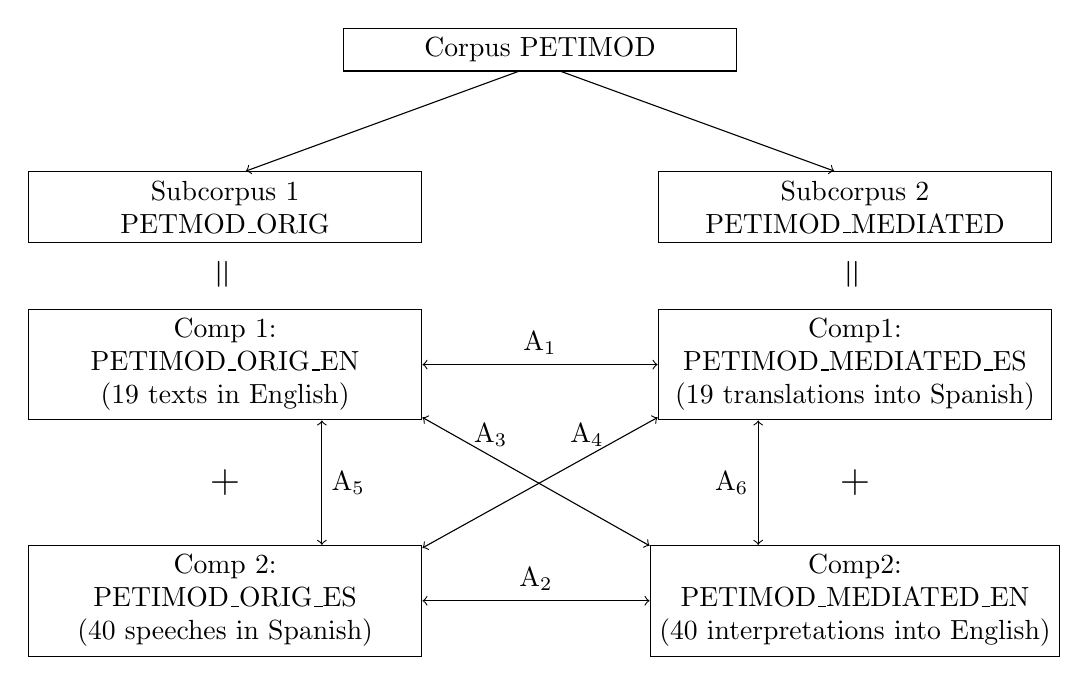
\begin{tikzpicture}[
		align=center,
		tips=proper,
		minimum width = 5cm
		]
		%nodes
		\node[draw, rectangle] at (4,7) (super){Corpus PETIMOD};
		\node[draw, rectangle] at (0,5) (sub1){Subcorpus 1\\PETMOD\_ORIG};
		\node[draw, rectangle] at (0,3) (comp11){Comp 1:\\PETIMOD\_ORIG\_EN\\(19 texts in English)};
		\node[draw, rectangle] at (0,0) (comp12){Comp 2:\\PETIMOD\_ORIG\_ES\\(40 speeches in Spanish)};
		\node[draw, rectangle] at (8,5) (sub2){Subcorpus 2\\PETIMOD\_MEDIATED};
		\node[draw, rectangle] at (8,3) (comp21){Comp1:\\PETIMOD\_MEDIATED\_ES\\(19 translations into Spanish)};
		\node[draw, rectangle] at (8,0) (comp22){Comp2:\\PETIMOD\_MEDIATED\_EN\\(40 interpretations into English)};
		\node at (0,4.1) {\Large \rotatebox{90}{$\,=$}};
		\node at (0,1.5) {\Large +};
		\node at (8,4.1) {\Large \rotatebox{90}{$\,=$}};
		\node at (8,1.5) {\Large +};
		%arrows
		\draw[->] (super.225) -- (sub1.60);
		\draw[->] (super.314) -- (sub2.120);
		\draw[<->] (comp11) edge node[above]{A$_1$} (comp21);
		\draw[<->] (comp12) edge node[above]{A$_2$} (comp22);
		\draw[<->] (comp11.345) edge node[pos=.3,above]{A$_3$} (comp22.165);
		\draw[<->] (comp12.15) edge node[pos=.7,above]{A$_4$} (comp21.195);
		\draw[<->] (comp11.330) edge node[minimum width=10pt,right]{A$_5$} (comp12.30);
		\draw[<->] (comp21.210) edge node[minimum width=10pt,left]{A$_6$} (comp22.150);
	\end{tikzpicture}
}
\caption{
PETIMOD subcorpora and envisaged comparisons.
}
\label{fig:corpas:1}
\end{figure}



\section{Methodology}\label{sec:corpas:4}

In order to study shifts in translated speeches and interpretations, we have focussed on NEs and extraction techniques. Named entity recognition (NER) is the task of identifying and categorising key information or real-world objects (entities) in text. In NLP, a NE is a real-world “object” that is assigned a name (e.g., \textit{Donald Trump}, \textit{United States}, \textit{The Foreign Office}, \textit{World Health Organisation}, etc.). 

For this study both automatic and manual extraction of NEs were performed. Both precision and recall were calculated in order to assess the system’s performance. Then, a corpus-based study of NEs in the translated and interpreted components was carried out.


\subsection{Automatic named entity recognition}\label{sec:corpas:4.1}

Similarly to other models trained on a Wikipedia-based corpus (\cite{NothmanEtAl2013}), for this paper we have used the VIP\footnote{VIP (Voice-text integrated system for InterPreters) is a hub of online resources and computer-assisted tools for interpreters created by the research group Lexytrad of the University of Malaga. VIP includes a suit of interpreting-related tools with a NER module and its own annotation scheme. The platform can be accessed here: \url{http://www.lexytrad.es/VIP/index_en.php}.} NER annotation scheme, that distinguishes four entity types: \textsc{per} (named person or family), \textsc{loc} (name of politically or geographically defined locations, e.g., cities, countries, regions, rivers, lakes, seas, mountains), \textsc{org} (named corporate, governmental or other organisational entities) and \textsc{misc} (miscellaneous entities, e.g., laws, events, languages, products, work of art, etc.). In order to extract and identify NEs automatically, a script\footnote{Authors would like to express their gratitude to Mr Francisco Javier Lima for writing the script used in this paper, which has been integrated in the VIP NER functionality.}  has been programmed based on the VIP module for NE chunking, extraction, and identification. See \figref{fig:corpas:2} for a screenshot of the Excel file generated by the script.

\begin{figure}
%%please move the includegraphics inside the {figure} environment
\includegraphics[width=\textwidth]{figures/a8NLPenhancedShiftAnalysisofNamedEntitiesinanEnglishSpanishIntermodalZoteroformatted-img002.png}
 

\caption{
English NEs file automatically retrieved by the VIP script.
}
\label{fig:corpas:2}
\end{figure}

VIP integrates spaCy\footnote{\url{https://spacy.io/}.} (a free open-source library in Python). VIP provides a user-friendly interface and allows importing NEs into an Excel file. Pre-trained spaCy models rather than custom-made NER models were used. The two pre-trained spaCy models used -- es\_core\_news\_lg (Spanish) and en\_core\_web\_lg (English) -- differ in the degree of granularity of the NER annotation scheme. The Spanish model recognises four categories (\textsc{per, loc, org} and \textsc{misc}), whereas the English model recognises twelve additional types of entities: \textsc{ordinal} (e.g., \textsuperscript{s}\textsuperscript{t}, \textit{second}), \textsc{date} (\textit{13 October}, \textit{2019}), \textsc{gpe} (countries, cities and states, e.g., \textit{Madrid}), \textsc{cardinal} (\textit{102}, \textit{67.5}), \textsc{norp} (nationalities, religious or political groups, e.g. \textit{Democrats}), \textsc{fac} (buildings, airports, highways, bridges, etc., e.g. \textit{Golden Gate}), \textsc{percent} (percentage, including \%), \textsc{product} (objects, vehicle, foods, etc., e.g. \textit{Toyota}), \textsc{law} (laws, directives, regulations, etc.), \textsc{quantity} (measurements of weight, distance, etc., e.g., \textit{hectare}), \textsc{money} (e.g., \textit{cents}, \textit{dollars}), \textsc{time} (times smaller than a day), and \textsc{language} (e.g., \textit{Spanish}). For this reason, English categories have been simplified. Thus, akin to the Spanish model, \textsc{fac} and \textsc{gpe} have been subsumed under the category \textsc{loc} and the rest have been grouped under \textsc{misc}.

Precision has been calculated to measure how well our NER system performs. Precision is defined as the fraction of relevant instances among all retrieved instances, i.e. the total number of relevant NEs retrieved divided by the number of all NEs retrieved (correctly and incorrectly identified by the model). 

\begin{equation*}
\mathit{Relevant}\,\mathit{NEs}=\mathit{Total}\,\mathit{number}\,\mathit{of}\,\mathit{correctly}\, \mathit{retrieved}\,\mathit{NEs}-\mathit{Errors}
\end{equation*}

\begin{equation*}
\mathit{Precision}=\text{~}\frac{\mathit{Relevant}\,\mathit{NEs}}{\mathit{Total}\,\mathit{number}\, \mathit{of}\,\mathit{extracted}\,\mathit{NEs}}
\end{equation*}

For calculating the above formula, it was necessary to manually assign the retrieved NEs to three categories: (a) segments which were correctly identified as NEs (“Correct ID”), (b) segments wrongly identified as NEs (“Wrong ID”), (c) and segments correctly identified as NEs but wrongly labelled (“Wrong Class”). 

NER performance has been calculated in terms of precision for both languages. Two levels of analysis have been established. The first level takes all NEs correctly identified as relevant, irrespective of their classification. For instance, the non-entity sequence [\textit{Articles 20(2)(b}], retrieved as NE by the system, would be classified as an error, whereas the retrieved sequence [\textit{2004/18/EC}] would be considered as relevant (correctly identified) whether it has been tagged correctly (\textsc{misc}) or not (\textsc{org}). The mathematical formula for Level 1 is as follows:

\begin{equation*}
    Precision = \frac{(Correct\,ID + Wrong\, Class)}{(Correct\,ID + Wrong\,ID + Wrong\,Class)}
\end{equation*}

\tabref{tab:corpas:4} presents results for this wider category of relevant NEs.

\begin{table}
\begin{tabularx}{\textwidth}{Qrr} 
\lsptoprule
& {\bfseries English} & {\bfseries Spanish}\\
\midrule
{\bfseries NEs retrieved} & 1,726 & 1,183\\
Correct identification & 1042 & 456\\
Wrong identification & 522 & 576\\
Wrong class & 162 & 151\\
{\bfseries Errors} & 684 & 727\\
Relevant NEs retrieved & 1204 & 607\\
{\bfseries Precision} & 0.697 & 0.513\\
\lspbottomrule
\end{tabularx}
\caption{
NER performance in terms of precision (Correct ID + Wrong Class).
}
\label{tab:corpas:4}
\end{table}

A further level of analysis is achieved by discriminating between NEs correctly identified and correctly tagged (for instance, [\textit{2004/18/EC}] correctly identified as NE and classified as \textsc{misc}) and NEs correctly identified but wrongly tagged (for instance NE [\textit{2004/18/EC}] classified as \textsc{org}). The formula below allows refining results by considering wrong-labelled NEs as errors (see \tabref{tab:corpas:5}).

\begin{equation*}
    Precision = \frac{(Correct\,ID)}{(Correct\,ID + Wrong\,ID + Wrong\,Class)}
\end{equation*}

\begin{table}
\begin{tabularx}{\textwidth}{Qrr} 
\lsptoprule
& {\bfseries English} & {\bfseries Spanish}\\
\midrule
{\bfseries NEs retrieved} & 1,726 & 1,183\\
Correct identification & 1042 & 456\\
Wrong identification & 522 & 576\\
Wrong class & 162 & 151\\
{\bfseries Errors} & 522 & 576\\
Relevant NEs retrieved & 1,042 & 456\\
{\bfseries Precision} & 0.603 & 0.385\\
\lspbottomrule
\end{tabularx}
\caption{
NER performance in terms of precision (Correct ID).
}
\label{tab:corpas:5}
\end{table}


\subsection{Manual named entity extraction}\label{sec:corpas:4.2}

In order to assess the performance of the system in terms of recall, it was necessary to identify and extract NEs manually for both languages. Recall is the fraction of retrieved instances among all relevant instances, i.e. it refers to the total number of relevant NEs retrieved versus the total number of relevant NEs found manually in our corpora. The idea was to delve into word lists generated by a corpus management tool, so we could identify NEs in the documents that had not been automatically recognised by our system. The sum of both types of NEs (automatically recognised and manually extracted) would bring the total number of relevant NEs in the corpus. The formula used to calculate recall is presented below:

\begin{equation*}
\mathit{Recall}=\text{~}\frac{\mathit{Relevant}\,\mathit{NEs}\,\mathit{extracted}}{\mathit{Total}\,\mathit{number}\,\mathit{of}\,\mathit{relevant}\,\mathit{NEs}\,in\,\mathit{the}\,\mathit{corpus}}
\end{equation*}

The selected corpus management platform was Sketch Engine, the same tool used for corpus statistics in \sectref{sec:corpas:3.1}. Sketch Engine was chosen for two reasons: it features European Parliament corpora \citep{Ustaszewski2019} and its interface allows for swift change when working with several subcorpora simultaneously. We uploaded the plain-text files for each of the four components of our intermodal corpus as four different monolingual comparable corpora, using the “New Corpus” functionality in the menu “Select Corpus $\rightarrow$ My Corpora”. 

Then, a starting point for manual NER was the wordlist generator of Sketch Engine, which was used in each component. We chose to compose a list of nouns filtered by two stopword lists (one for each language).\footnote{Stopword lists were directly copied and pasted from \url{http://members.unine.ch/jacques.savoy/clef/index.html}. The interjection “ehm”, used in the transcription conventions for representing hesitation in speech, was also added to the stopword list.} In Sketch Engine, this can be done in the “Advanced” tab of the wordlist menu, under the heading “Exclude these words”; the list has to be pasted manually, with one word per line. The PETIMOD\_MEDIATED\_EN subcorpus, for example, yielded a list of 643 nouns (e.g., \textit{Commission}, \textit{situation}, \textit{petitioner}, \textit{problem}, etc.).

Once the wordlist was generated (Wordlist 1), we had a basic frequency list which contained some nouns that could be used to refine the automatic NER, such as committee (22 occurrences), directive (16), agreement (13), group (11), plan (10), fund (9), etc. 
Then, a second wordlist (Wordlist 2) was created by sorting the nouns alphabetically and filtering out those which were neither semantically nor frequency-wise relevant (e.g. \textit{angle}, 1) or which had been correctly recognised by the automatic NER (e.g. \textit{Aguilar}, 1). Although Sketch Engine did not allow for alphabetical sorting of the wordlist, nor for complete visualisation of the results in one column (the maximum is 500), it was possible to download the data in a CSV file and order the words by using the corresponding Excel function.

The next step was to search for the nouns in the wordlist manually. To this end, we opened a new window of concordances in Sketch Engine to directly search for the occurrences of each noun in the corpus. At this point, some basic functions of concordance search, such as alphabetical sort by context (left and right), file view, and wildcard search, were also used for easier and faster identification of new entities. Wildcard search proved especially useful in combination with the wordlist, as in some cases looking for lexical roots made it possible to inspect several instances of the list at once. For instance, a search for [\textit{*omission*}] retrieved up to three instances of the wordlist simultaneously (\textit{Commission}, \textit{commission}, and \textit{commissioner}).

Apart from wordlist frequency, institutionalisation was the second criterion for identifying relevant NEs. In this case, coverage in Eur-lex,\footnote{\url{https://eur-lex.europa.eu/}.}  IATE\footnote{\url{https://iate.europa.eu/home}.}  and/or TermCoord’s Glossary Links\footnote{A database of more than 8,000 glossaries managed by the Terminology Coordination Unit of the EP Directorate-General for Translation (\url{https://termcoord.eu/glossarylinks/}).}  was taken as a reference (see \figref{fig:corpas:3}).

\begin{figure} 
%%please move the includegraphics inside the {figure} environment
\includegraphics[width=\textwidth]{figures/a8NLPenhancedShiftAnalysisofNamedEntitiesinanEnglishSpanishIntermodalZoteroformatted-img003.png}

\caption{Example of manual NER using institutional criteria. The consulted NE (“EU law”) had not been automatically recognised.}
\label{fig:corpas:3}
\end{figure}

Following these criteria, new NEs were extracted from the concordances in each component and saved in an Excel file. Some examples of further relevant NEs manually extracted were \textit{Directorate-General for the Mar Menor} (\textsc{org}, PETIMOD\_MEDIATED\_EN), \textit{Acuerdo de Asociación Económica} (\textsc{misc}, PETIMOD\_MEDIATED\_ES), \textit{municipality of Real} (\textsc{loc}, PETIMOD\_ORIG\_EN) and \textit{Directiva de inundaciones} (\textsc{misc}, PETIMOD\_ORIG\_ES), among others. 

Finally, NER performance has been calculated in terms of recall for both languages. As in the case of precision, two granular levels of analysis have been used. The first level takes all NEs correctly identified by the script as relevant, irrespective of their classification (see \sectref{sec:corpas:4.1}). For these calculations, it was necessary to sum the manually retrieved NEs for each component, combining and sorting them by language.

\begin{table}
\begin{tabularx}{\textwidth}{Qrr} 
\lsptoprule
& {\bfseries English} & {\bfseries Spanish}\\
\midrule
{\bfseries Total no. of relevant NEs} & 1,557 & 896\\
Relevant NEs retrieved automatically & 1,204 & 607\\
Relevant NEs retrieved manually & 353 & 289\\
{\bfseries Recall} & 0.773281 & 0.677455\\
\lspbottomrule
\end{tabularx}
\caption{
NER performance in terms of recall (Correct ID + Wrong Class).
}
\label{tab:corpas:6}
\end{table}

A further level of recall analysis is achieved by discriminating between NEs correctly identified and correctly tagged by the automatic script (relevant) and NEs correctly identified but wrongly tagged (not relevant). This allows refining recall results by excluding wrong-labelled NEs from calculation. 

\begin{table}
\begin{tabularx}{\textwidth}{Xrr} 
\lsptoprule
& {\bfseries English} & {\bfseries Spanish}\\
\midrule
{\bfseries Total no. of relevant NEs} & 1,075 & 745\\
Relevant NEs retrieved automatically & 1,042 & 456\\
Relevant NEs retrieved manually & 353 & 289\\
{\bfseries Recall} & 0.969302 & 0.612080\\
\lspbottomrule
\end{tabularx}
\caption{
NER performance in terms of recall (Correct ID).
}
\label{tab:corpas:7}
\end{table}


\subsection{Corpus-based analysis}\label{sec:corpas:4.3}

For the corpus-based analysis described in this section, all relevant NEs in the Excel files (correctly identified, correctly identified but mislabelled, and manually extracted) were prepared by listing them together in a new file, manually sorting them by category and language.  \figref{fig:corpas:4} below shows the two columns for the \textsc{per} category (English and Spanish), the first one attending to the VIP annotation scheme order described above.

Once all NEs were prepared, the next step was analysing the observable shifts in their translation and/or interpretation. We decided to perform the shift analysis both in the EN>ES translation (components PETIMOD\_ORIG\_EN vs. PETIMOD\_MEDIATED\_ES, or direction A1 in \figref{fig:corpas:1}) and in the ES>EN interpretation (components PETIMOD\_ORIG\_ES vs. PETIMOD\_MEDIATED\_EN, or direction A2 in \figref{fig:corpas:1}). The reasons for this decision were two: it comprised all the different components in our corpora, and the cross-comparison of translation and interpreting analysis was expected to show interesting findings.

\begin{figure}
%%please move the includegraphics inside the {figure} environment
\includegraphics[width=\textwidth]{figures/a8NLPenhancedShiftAnalysisofNamedEntitiesinanEnglishSpanishIntermodalZoteroformatted-img004.png}
 

\caption{Screenshot of the Excel file with extracted PER NEs (English/Spanish).}
\label{fig:corpas:4}
\end{figure}

Provided that the raw material for analysis (i.e., the NEs) was already extracted, labelled, and sorted by language, the next three steps to be taken were: (1) contrasting them across languages to observe (possible) changes; (2) searching for them in the corpora in order to extract contextual exemplification of the shifts and identify their direction; (3) categorising the shifts. Step 1 could be done directly in the Excel file, underlining those units already analysed and/or not shifted. For Step 2, we prepared a mosaic-style panel of four windows, one for each uploaded component in Sketch Engine, in order to identify the directions and the exact alignment of the document in which the shift occurred (see \figref{fig:corpas:5}). A total of 142 shifts (69 for EN>ES translation, 73 for ES>EN interpretation) were identified and analysed. Regarding Step 3, the bottom-up transfer operations typology of \citet{Bernardini2016} was chosen to categorise the shifts (see \sectref{sec:corpas:5} for further description). The category was annotated next to the extracted concordances, in a table-like fashion. The Excel file for shift analysis included retrieved NEs and categorised shifts sorted by direction. As it can be inferred, the previous work with the entities in the automatic and manual NER phases was very helpful for this analysis, and allowed for quick identification and remembrance of the nature and direction of several shifts. Again, the institutional resources cited in \sectref{sec:corpas:4.2} (Eur-lex, IATE, Glossary Links) were occasionally used in combination with generic searches in Google and/or Wikipedia in order to gain insights into the possible motivations behind some of the shifts encountered.

\begin{figure}  
%%please move the includegraphics inside the {figure} environment
\includegraphics[width=\textwidth]{figures/a8NLPenhancedShiftAnalysisofNamedEntitiesinanEnglishSpanishIntermodalZoteroformatted-img005.png}
 

\caption{Four-window panel in Sketch Engine to track shifts in the corpus.}
\label{fig:corpas:5}
\end{figure}



\section{Shift analysis and results}\label{sec:corpas:5}

The term “shifts” commonly refers to “changes which occur or may occur in the process of translating [and interpreting]” (\citealt[269]{BakkerEtAl2009}). Shifts of translation (and interpreting) can be distinguished from the systemic differences which exist between source and target languages and cultures. Systemic differences, which pertain to the level of competence, are part of the opening conditions for translation (and interpreting). Shifts, on the other hand, result from attempts to deal with systemic differences (ibid). In this study, only NEs that experienced shifts during translation/interpreting were analysed, whereas translations/interpretations where no shifts in NEs occurred were ignored. As stated in the previous section, the bottom-up transfer operations typology from \citet[140]{Bernardini2016}, used to categorise shifts in the intermodal corpus EPTIC, was chosen for this analysis. It includes register shifts (either upwards or downwards), quantitative meaning shifts (contraction, expansion, clarification, broadening), and transformational meaning shifts (partial and total), as well as cases akin to normalisation.\footnote{For the sake of clarity, the original name of this category was rephrased for this chapter (from “more collocational” to “normalisation”).} In the next paragraphs, each of these categories will be described and illustrated with examples from our corpus.\footnote{We followed the same conventions of \citet[140]{Bernardini2016}. The underlined NE in the source roughly corresponds to the NE or segment in the target (in angle brackets).} However, as Bernardini (ibid.) puts it:

\begin{quote}
As often happens with language in use, some instances were impossible to assign indisputably to one category only. In these cases a decision was made based on a close reading of the co-text and, inevitably, intuition as to the main reason for making a certain choice. \citep[140]{Bernardini2016} 
\end{quote}

The first type of shifts, categorised under “register” (up and down), could indeed be sometimes confused with contraction and expansion changes. Illustrating them with the use of acronyms helps establish a clear-cut separation between register shifts (formal) and meaning shifts. In example \REF{ex:corpas:1}, the acronym is avoided in the EN-ES direction, which increases the level of formality. It is shifted to the modifier \textit{de la Unión}, which in the Spanish eurolect can be considered even more formal than the alternative \textit{de la Unión Europea} because of its specificity. Exactly the same change can be further found in the same sentence (from \textit{EU Member States} to \textit{Estados Miembros de la Unión}).

\ea\label{ex:corpas:1}
%%1st subexample: change \ea\label{...} to \ea\label{...}\ea; remove \z  
%%further subexamples: change \ea to \ex; remove \z  
%%last subexample: change \z to \z\z 
Register up shift (EN-ES translation)
%\end{itemize}
\ea
The \underline{EU Delegation} in Japan and the authorities of EU Member States [PETIMOD\_ORIG\_EN]
\ex
La <Delegación de la Unión> en Japón y las autoridades de los Estados miembros de la Unión [PETIMOD\_MEDIATED\_ES]
\z
\z

On the contrary, in the ES-EN interpretation in example \REF{ex:corpas:2}, the acronym \textit{ENVI} is preferred instead of the denomination \textit{Comisión ENVI} (already shortened in the original). As the Spanish ISG always recommend the use of the word \textit{Comisión} when referring to these bodies (cf. \citealt{EU2021}: 172), this can be considered a shift which downgrades register. In fact, some shifts of the same nature can be observed in the surrounding verbs (\textit{pedimos \rightarrow$\,$ pass}, \textit{realice \rightarrow$\,$ carry out}).

\ea\label{ex:corpas:2}
%%1st subexample: change \ea\label{...} to \ea\label{...}\ea; remove \z  
%%further subexamples: change \ea to \ex; remove \z  
%%last subexample: change \z to \z\z 
Register down shift (ES-EN interpretation)
%\end{itemize}
\ea
le pedimos a la \underline{Comisión ENVI} que realice una visita [PETIMOD\_ORIG\_ES]
\ex
we should pass it on to <ENVI> and ask them to carry out a study... visit [PETIMOD\_MEDIATED\_EN]
\z
\z

Moving to quantitative meaning shifts, contraction implies changing from an informative detailed NE or NE sequence to a shorter and more under-defined equivalent \citep[141]{Bernardini2016}. Although the author does not put it explicitly, it can be deduced from the given examples that contraction and expansion are related, as the reduction (or addition) of meaning also conveys a reduction or addition in the number of words (ibid.). In example \REF{ex:corpas:3}, the English word referring to the region (\textit{Galicia}) is omitted in the Spanish translation, as it is (supposedly) not necessary for a standard Spanish reader.

\ea\label{ex:corpas:3}
%%1st subexample: change \ea\label{...} to \ea\label{...}\ea; remove \z  
%%further subexamples: change \ea to \ex; remove \z  
%%last subexample: change \z to \z\z 
Contraction shift (EN-ES translation)
%\end{itemize}
\ea
in an existing business park, on a green field plot, in Curtis-Teixeiro, \underline{La Coruña , Galicia, Spain}. [PETIMOD\_ORIG\_EN]
\ex
en un parque de actividades económicas ubicado en un terreno no urbanizado de Curtis-Teixeiro <(La Coruña, España)> [PETIMOD\_MEDIATED\_ES]
\z
\z

A similar example, but this time of expansion, could be extracted from the ES-EN direction. Here we also have a \textsc{loc}  NE referred to a quite specific Spanish area (\textit{Campo de Cartagena}), but the interpreter’s decision is the opposite one: adding the modifier \textit{region} to specify the nature of the named entity, thus increasing the number of words.

\ea\label{ex:corpas:4}
%%1st subexample: change \ea\label{...} to \ea\label{...}\ea; remove \z  
%%further subexamples: change \ea to \ex; remove \z  
%%last subexample: change \z to \z\z 
Expansion shift (ES-EN interpretation)
%\end{itemize}
\ea
él estaba contentísimo con el modelo agrícola del \underline{Campo de Cartagena} [PETIMOD\_ORIG\_ES]
\ex
they were very happy with the agricultural model in the <Campo de Cartagena region> [PETIMOD\_MEDIATED\_EN]
\z
\z

Like expansion shifts, clarifications are instances of addition, in which meanings that are implicit in the sources are made explicit in the targets. As a rule of thumb, \citet[140]{Bernardini2016} states that “in the case of clarification words used are more explicit, whereas in the case of expansion there is also an increase in the number of words (though admittedly the difference is not always clear-cut).” For improved distinction, it could be added that clarification seemingly implies adding \textit{less} words that any expansion would. Again, the \textsc{loc} label provides a suitable example in the EN-ES translation. In example \REF{ex:corpas:5} the unit \textit{municipality of Real}, which initially refers to a geopolitical entity and could imply demanding information from any office contained in these borders, is shifted to a more explicit reference (\textit{Ayuntamiento de Real} or town hall). Interestingly, by performing this operation, the nature of the NE is also shifted (from \textsc{loc} to \textsc{org}).

\ea\label{ex:corpas:5}
%%1st subexample: change \ea\label{...} to \ea\label{...}\ea; remove \z  
%%further subexamples: change \ea to \ex; remove \z  
%%last subexample: change \z to \z\z 
Clarification shift (EN-ES translation)
%\end{itemize}

\ea
the Environmental Inspection Service requested the \underline{municipality of Real} to inform [PETIMOD\_ORIG\_EN]
\ex
En 2012, el Servicio de Inspección Medioambiental pidió al <Ayuntamiento de Real> información [PETIMOD\_MEDIATED\_ES]
\z
\z

The third possible case of quantitative meaning shift is broadening, or generalisation through vaguer or emptier terms. In example \REF{ex:corpas:6}, two \textsc{per}  NEs are generalised through the common, more neutral noun \textit{petitioners}. This is a quite prototypical example, as additionally the first \textsc{per} (\textit{Eduardo Salazar Ortuño}) is not one of the petitioners, but a lawyer who is present on behalf of them (this is contextual information which can be found in the corpus some interventions before). Other aspects worth mentioning are the double nature of the shift and the extended broadening phenomena in the two \textsc{misc} NEs \textit{dos minutos}, which are suppressed in favour of the more general idea conveyed by \textit{conclude}.

\ea\label{ex:corpas:6}
%%1st subexample: change \ea\label{...} to \ea\label{...}\ea; remove \z  
%%further subexamples: change \ea to \ex; remove \z  
%%last subexample: change \z to \z\z 
Broadening shift (ES-EN interpretation)
%\end{itemize}
\ea
para concluir esta petición le daríamos la palabra por dos minutos al señor \underline{Eduardo Salazar Ortuño} // y luego le daríamos dos minutos más al señor \underline{José Luis Álvarez-Castellanos Rubio} [PETIMOD\_ORIG\_ES]
\ex
let's close the debate on that and we will conclude this point by giving the floor back to <our two petitioners> [PETIMOD\_MEDIATED\_EN]
\z
\z

Transformational shifts include two different grades (partial and total). Partial transformation involves a reformulation with approximately the same co-textual meaning, but using an unrelated expression with a different out-of-context meaning \citep[142]{Bernardini2016}. Again, the ES-EN interpretation provides a prototypical example of partial transformation. The collocation \textit{flourishing ecosystem} in example \REF{ex:corpas:7} does not convey the same specialised meaning as \textit{Zona de Especial Conservación}, but serves as equivalent in the context of the inversion operated in the target sentence. As already observed in example \REF{ex:corpas:6}, the shift affects more than one particular NE and can be analysed even at the sentence level.

\ea\label{ex:corpas:7}
%%1st subexample: change \ea\label{...} to \ea\label{...}\ea; remove \z  
%%further subexamples: change \ea to \ex; remove \z  
%%last subexample: change \z to \z\z 
Partial transformation shift (ES-EN interpretation)
%\end{itemize}
\ea
en la cuenca del Mar Menor la Red Natura 2000 es una etiqueta formal que no responde a una gestión eficiente de lo que sería una \underline{Zona de Especial Conservación} [PETIMOD\_ORIG\_ES]
\ex
Natura 2000 is an official label that should lead to efficient management of what should be a <flourishing ecosystem> [PETIMOD\_MEDIATED\_EN]
\z
\z

Total transformation, on the other hand, may sometimes override the limits of equivalence and fall closer to the notion of translation error (see for example \citealt{Hurtado2017}). In example \REF{ex:corpas:8}, the translator seems to have looked for the real (and very different) equivalent of the generic NE underlined in \REF{ex:corpas:8}, but has made a mistake in the process (\textit{Consejería de Turismo y Cultura} instead of \textit{Consejería de Turismo, Cultura y Medio Ambiente}).\footnote{See \url{https://www.borm.es/services/anuncio/ano/2017/numero/3482/pdf?id=757271}. In fact, the name of the supervising office is now “Consejería de Agua, Agricultura, Ganadería, Pesca y Medio Ambiente” (\url{https://administracion.gob.es/pagFront/espanaAdmon/directorioOrganigramas/fichaUnidadOrganica.htm?idUnidOrganica=123379 & origenUO=comunidadesAutonomas & comunidadesAutonomas=true & volver=comunidadesAutonomas & idCCAA=14\#.X-DOye1Ce00}).} This is a very similar case to the one illustrated by \citet[142]{Bernardini2016}, in which an error is produced in the search of a salient collocation (here, a NE) in the target language.

%% the last url leads to a wrong page, maybe wrong url or the page is moved?

\ea\label{ex:corpas:8}
%%1st subexample: change \ea\label{...} to \ea\label{...}\ea; remove \z  
%%further subexamples: change \ea to \ex; remove \z  
%%last subexample: change \z to \z\z 
Total transformation shift (EN-ES translation)
%\end{itemize}
\ea
the creation of a specific Directorate-General for the Mar Menor, within the \underline{regional Department for the Environment} [PETIMOD\_ORIG\_EN]
\ex
la creación de una Dirección General del Mar Menor, dentro de la <Consejería de Turismo y Cultura> [PETIMOD\_MEDIATED\_ES]
\z
\z

The last shift category presented in this typology is normalisation. In the words of Bernardini \citep[142]{Bernardini2016}, here “the difference from source to target seems to be one of \textit{collocationality}: i.e., the inherent motivation for using a certain turn of phrase seems to be its salience as a phrase, or status as a collocation, in the target language.” In this study, however, the analysed normalisation shifts are not performed on collocations, but on multi-word terms or NEs, such as the ones in example \REF{ex:corpas:9}. In this translation, a subtle shift in a preposition (\textit{National Assembly in France} \rightarrow$\,$ \textit{Asamblea Nacional de Francia}) reveals a more frequent\footnote{For example, a search in the Spanish reference corpus CORPES (\url{https://webfrl.rae.es/CORPES/view/inicioExterno.view})  yields five results against zero.} multi-word term in the target language than \textit{Asamblea Nacional en Francia}.

\newpage
\ea\label{ex:corpas:9}
%%1st subexample: change \ea\label{...} to \ea\label{...}\ea; remove \z  
%%further subexamples: change \ea to \ex; remove \z  
%%last subexample: change \z to \z\z 
Normalisation shift (EN-ES translation)
%\end{itemize}
\ea
on 16 February 2019, the \underline{National Assembly in France} has adopted the law of programming 2019--2022 and the justice reform [PETIMOD\_ORIG\_EN]
\ex
la <Asamblea Nacional de Francia> adoptó el 16 de febrero de 2019 la ley de programación 2019--2022 y la reforma judicial [PETIMOD\_MEDIATED\_ES]
\z
\z



\section{Discussion}\label{sec:corpas:6}

In this section, the overall results of our analysis are discussed, focusing on three different quantifications for both translation and interpreting: 1) distribution of the type of shifts retrieved; 2) distribution of the labels of the shifted entities; and 3) the detailed shift entity relationship with all the subcategories of shifts as described above. Then, we will relate our findings to results reported in related literature on intermodal corpora.

\figref{fig:corpas:6} quantifies certain tendencies within English-Spanish translations and Spanish-English interpretations in the Committee on Petitions. The most prominent shifts are quantitative shifts (75 instances in both language pairs) and register shifts (33), followed by transformational shifts (18) and normalisations (16). There is a predominance of register shifts in EN-ES translations (20 against 13) and a fairly more balanced number in the case of quantitative meaning shifts (36 against 39). Transformational meaning shifts are more numerous on ES-EN interpretations (2 against 16); inversely, normalisations are more present in the translations into Spanish (11 against 5).

\begin{figure}
%\includegraphics[width=\textwidth]{figures/a8NLPenhancedShiftAnalysisofNamedEntitiesinanEnglishSpanishIntermodalZoteroformatted-img006.png}
\scalebox{.8}{
 \begin{tikzpicture}
            \begin{axis}[
                xbar,
                xmin=0,
                xmax=40,
                axis lines*=left,
                width=\textwidth,
                height=7cm,
                symbolic y coords={Register,{Meaning (quantitative)},{Meaning (transformation)},Normalisation},
                ytick=data,
                nodes near coords,
                nodes near coords align = horizontal,
                legend pos = north east,
                reverse legend,
                point meta=rawx
                ]
                 \addplot+[lsDarkBlue,fill=lsDarkBlue,]
                    coordinates {
                   (20,Register)
		(36,{Meaning (quantitative)})
		(2,{Meaning (transformation)})
		(11,Normalisation)
                };
                \addplot+[lsMidOrange,fill=lsMidOrange,]
                      coordinates {
                   (13,Register)
		(39,{Meaning (quantitative)})
		(16,{Meaning (transformation)})
		(5,Normalisation)
                };

                \legend{EN-ES translations,ES-EN interpretations}
            \end{axis}
        \end{tikzpicture} 
}
\caption{
Type of shifts distribution.
}
\label{fig:corpas:6}
\end{figure}

\newpage
\figref{fig:corpas:7} shows the distribution of shifted NEs per label, as illustrated in \sectref{sec:corpas:3} of this chapter. \textsc{misc} entities are the most frequent (58), closely followed by \textsc{org} (51); \textsc{loc} (22) and \textsc{per} (11) are considerably less represented in the shifts. The miscellaneous entities are more subject to shifts in the interpretations into English (26 against 32); conversely, organisational entities are prone to shifts in the translations into Spanish (30 against 21). The number of locations remains fairly equal in both directions (12 against 10). Finally, shifts in named persons are almost inexistent in EN-ES translations (only 1 result) in comparison to ES-EN interpretations (10).

\begin{figure}

%\includegraphics[width=\textwidth]{figures/corpas_shifted_entities.png}
\begin{tikzpicture}
            \begin{axis}[
                xbar,
                xmin=0,
                xmax=40,
                axis lines*=left,
                width=\textwidth,
                height=7cm,
                symbolic y coords={MISC,LOC,ORG,PER},
                ytick=data,
                nodes near coords,
                nodes near coords align = horizontal,
                legend pos = north east,
                reverse legend,
                point meta=rawx
                ]
                 \addplot+[lsDarkBlue,fill=lsDarkBlue,]
                    coordinates {
                   (32,MISC)
		(10,LOC)
		(21,ORG)
		(10,PER)
                };
                \addplot+[lsMidOrange,fill=lsMidOrange,]
                      coordinates {
                   (26,MISC)
		(12,LOC)
		(30,ORG)
		(1,PER)
                };

                \legend{EN-ES translations,ES-EN interpretations}
            \end{axis}
        \end{tikzpicture}

\caption{
Shifted entities distribution.
}
\label{fig:corpas:7}
\end{figure}

In \tabref{tab:corpas:8}, \ref{tab:corpas:9} and \ref{tab:corpas:10}, the two types of data commented above (type of shifts and type of entities) are cross-related and broken down into the nine shift subcategories used for this study.

\begin{table}
\begin{tabularx}{\textwidth}{Qrrrrr}

\lsptoprule

{\bfseries Type of shift} & {\bfseries \textsc{per}} & {\bfseries \textsc{org}} & {\bfseries \textsc{loc}} & {\bfseries \textsc{misc}} & {\bfseries Total}\\
\midrule
Register up & 0 & 6 & 3 & 10 & 19\\
Register down & 0 & 0 & 1 & 0 & 1\\
Contraction & 0 & 4 & 2 & 9 & 15\\
Clarification & 1 & 0 & 2 & 1 & 4\\
Expansion & 0 & 9 & 1 & 4 & 14\\
Broadening & 0 & 1 & 1 & 1 & 3\\
Partial transformation & 0 & 0 & 0 & 1 & 1\\
Total transformation & 0 & 1 & 0 & 0 & 1\\
Normalisation & 0 & 9 & 2 & 0 & 11\\
\lspbottomrule
\end{tabularx}
\caption{
Detailed shift-entity relationship (EN-ES translations)
}
\label{tab:corpas:8}
\end{table}


\begin{table}
\begin{tabularx}{\textwidth}{Qrrrrr}

\lsptoprule

{\bfseries Type of shift} & {\bfseries \textsc{per}} & {\bfseries \textsc{org}} & {\bfseries \textsc{loc}} & {\bfseries \textsc{misc}} & {\bfseries Total}\\
\midrule
Register up & 0 & 0 & 0 & 1 & 1\\
Register down & 0 & 5 & 2 & 5 & 12\\
Contraction & 4 & 2 & 1 & 3 & 10\\
Clarification & 0 & 1 & 0 & 2 & 3\\
Expansion & 1 & 0 & 1 & 0 & 2\\
Broadening & 3 & 6 & 6 & 9 & 24\\
Partial transformation & 1 & 1 & 0 & 6 & 8\\
Total transformation & 1 & 1 & 0 & 6 & 8\\
Normalisation & 0 & 5 & 0 & 0 & 5\\
\lspbottomrule
\end{tabularx}
\caption{
Detailed shift-entity relationship (ES-EN interpretations)
}
\label{tab:corpas:9}
\end{table}

\tabref{tab:corpas:10} contrasts the subcategories of shifts encountered in both directions (EN-ES translations vs. ES-EN interpretations).

\begin{table}
\begin{tabularx}{\textwidth}{Qrr}

\lsptoprule

{\bfseries Type of shift} & {\bfseries EN-ES translation} & {\bfseries ES-EN interpretation}\\
\midrule
Register up & 19 & 1\\
Register down & 1 & 12\\
Contraction & 15 & 10\\
Clarification & 4 & 3\\
Expansion & 14 & 2\\
Broadening & 3 & 24\\
Partial transformation & 1 & 8\\
Total transformation & 1 & 8\\
Normalisation & 11 & 5\\
\lspbottomrule
\end{tabularx}
\caption{
Comparison of shift subcategories in both directions
}
\label{tab:corpas:10}
\end{table}

In this comparison, major differences can be found which help characterising the shifting profile of each type of transfer separately. It appears that, when operating with named entities:

\begin{itemize}
\item 
English-Spanish translations tend to upgrade register (19), change meaning by contracting (15) and expanding (14), and to normalise multi-word terms (11).

\item 
Spanish-English interpretations, contrarily, tend to downgrade register (12), change meaning by contracting (10) and broadening (24), and to present more transformations, be they partial (8) or total (8). 

\end{itemize}

In general, the results show clear differences in the nature of shifts between EN-ES translations and ES-EN interpretations in the Petitions Committee. Translations from English into Spanish present more frequently register (e.g. \textit{RAMSAR} \rightarrow$\,$ \text{Convención de Ramsar})\footnote{These examples were extracted from the most common NE categories in each case according to the correlation \tabref{tab:corpas:8} and \tabref{tab:corpas:9}.} and normalisation shifts (e.g. \textit{Government of Valencia's Ministry of Agriculture} \rightarrow$\,$ \textit{Consejería de Agricultura de la Generalitat Valenciana}). In the case of register, practically all changes are upwards (\textit{Bulgarian Ministry of Environment and Water} \rightarrow$\,$ \textit{Ministerio Búlgaro de Medio Ambiente y Recursos Hídricos}), as opposed to the downward tendency of the shifts in the interpretations into English (\textit{Comisión de Medio Ambiente del Parlamento Europeo} \rightarrow$\,$ \textit{ENVI Committee}). The fact that Spanish translators tend to be more formal than English interpreters was a previous intuition confirmed by the data, similarly to the results obtained by \citet[143--144]{Bernardini2016} in her comparative analysis of Italian-English translations. Moreover, results in normalisation bring a new perspective to previous studies, as this is a newly introduced shift category which focuses on changes in specialised multi-word terms instead of general-language collocations. In the case of Bernardini, results showed an increased tendency by Italian-English translators to insert general language collocations. Our data show that normalisation of specialised phraseology is preferred when translating into the Romance language (Spanish) instead.

Moving on to quantitative meaning shifts, the interpretations present a slightly higher amount of them, although it must be specified that they are not of the same type in both directions and modes. While contraction and clarification are more or less equal, expansion prevails overwhelmingly in the EN-ES translations, as in the example: \textit{Association for the Renaissance of Craiova (ARC)} \rightarrow$\,$ \textit{«Association for the Renaissance of Craiova » (ARC) (Asociación para el Renacimiento de Craiova)}. Inversely, broadening is much more numerous in the ES-EN interpretations (\textit{nueve\_mil\_seiscientas hectáreas ilegales} \rightarrow$\,$ \textit{considerable illegal construction}). Considering that broadening shifts could be regarded as a simplification feature, our results for the English-Spanish/Spanish-English pair are in line with the bidirectional English<>Italian study of \citet{BernardiniEtAl2016}, in which interpreters were found to simplify the input more than translators.

Finally, transformations are substantially more present in the ES-EN interpretations, where they are equally distributed among partial (\textit{Ley de Protección Integral del Mar Menor}  \textit{law for iterative protection of the Mar Menor}) and total (\textit{Planes de Ordenación de los Recursos Naturales} \rightarrow$\,$ \textit{natural protection ehm plans}). This is an interesting finding because it presents both similarities and divergences with previous intermodal studies. In \citet{Bernardini2016}, for example, transformations were also absent from English-Italian translations, but far more present in the other subcorpora, and the “partial” category outnumbered the “total” one. Although this could be the result of different conceptualisations by the researchers on what “transformation” means, it can also be argued that dissimilarities in transformational behaviour are connected to \citegen[1]{FerraresiMilicevic2017}  “cognitive and task-related constraints” characterising the translation and interpreting processes. In other words, the number and nature of the transformations operated by the translator and/or interpreter could be strongly dependent on factors beyond language direction or mode, such as the communicative situation in which they are working (e.g., whether the context is a plenary session of the Parliament or a Committee meeting) or even the topic of the source text.\footnote{These factors could also affect the degree of relation between total transformation shifts and translation/interpreting errors suggested in \sectref{sec:corpas:3}.}

Precisely with the goal of shedding some light on the connections between topic (or specialisation field, etc.) and the shifts involved in translation and interpreting, discussion should also centre on the shifted NEs label distribution shown in \figref{fig:corpas:7}. A clear majority of miscellaneous and organisational entities over locations and proper nouns of persons can be observed both in EN-ES translation and ES-EN interpreting. These results picture a cognitive domain of a rather political nature, in which parties, public platforms and similar organisations discussing policies and agreements are more important than the places where the problem occurred or the persons who complained in the first place. This perspective suits the function of the Committee on Petitions and points indeed towards a supranational way of making politics which permeates through the shifts encountered in translation and interpreting. What is more, a closer examination of \tabref{tab:corpas:8} and \ref{tab:corpas:9} reveals that there is a high degree of relationship between the frequencies of shifts and entities in both analysed directions and modes. For example, the frequent upward register shifts in EN-ES translation often occur in \textsc{misc} NEs (\textit{EU law} \rightarrow$\,$ \textit{Derecho de la Unión}), and the numerous broadening shifts in the ES-EN interpretations are usually operated on \textsc{org} NEs (\textit{departamentos de Ecología de la Universidad de Murcia} \rightarrow$\,$ \textit{the University of Murcia and its researchers}). Introducing this new parameter in the analysis of shifts could add a new variant to the conclusions of \citet{FerraresiEtAl2018} and lead us to hypothesise that simplification is a contingent feature which depends not only on the mediation mode and the source languages involved, but also on the topic of the source text. This is in line with calls for multifactorial research designs in empirical translation/interpreting studies (\cite{CorpasPastor2008}, \cite{DeSutterLefer2020}), since studies that take into account only one or two explanatory factors fall short of explaining the complexity of real-world translation/interpreting phenomena. Under this view, the analysed ES-EN interpretations of the Committee on Petitions would be more simplified than the EN-ES translations not just because they are an oral mediation performed into English, but also because the interpreters (consciously or not) would apply certain strategies aimed at approaching the content of their message to a broader audience than translation. This would imply neutralising or simplifying institutional-specific \textsc{misc} and \textsc{org} NEs (EU legislation, international agreements, public bodies, etc.), paradoxically the most unfamiliar in the ears of the European citizens who could also exercise their right of petition.

\section{Conclusion}\label{sec:corpas:7}

The study presented in this chapter can be regarded as innovative for various reasons. To the best of our knowledge, it is one of the first corpus-based studies which relies on translated and interpreted documents from the European Parliament Committee on Petitions. Secondly, it does not only build and employ a type of resource which is still in its infancy (intermodal corpora), but also introduces a new methodological layer through manual and state-of-the-art automatic named-entity recognition (the latter performed by spaCy). This approach added new aspects to the analysis of translation and interpreting shifts (a new shift category called “normalisation” and the possibility of correlating shifts to the semantic labels of the NEs involved), which in turn helped establish interesting findings in relation with previous studies (normalisation as a language-dependent feature of translation, transformation and simplification as contextual, topic-dependent features of interpreting).

\begin{sloppypar}
Our study presents some limitations, though. Concerning methodology, the suitability of the selected transcription conventions must be revised. Even though we introduced certain modifications to the system, some of the proposed features seem more adequate for multimodal corpora and are counterproductive when recognising NEs (consider for example the hesitation particle \textit{ehm} in \textit{the Socialist for ehm Party ehm from the ehm Murcia region}).  NE recognition and corpus-based shift analysis could also be extremely facilitated with the addition of an intermediate alignment phase to cope with terminology variation. In fact, monolingual terminological variation within NEs (e.g., \textit{The Court, Court of Justice of the European Union}, \textit{CJEU}, etc.) turned manual pairing into an exhausting job. As to NE labelling, a more fine-grained taxonomy is also needed for both languages, especially in the MISC category, where additional subtypes not available in the VIP scheme could be traced during the analysis (e.g. agreements like \textit{Ramsar} or quasi-legal documents such as \textit{Estrategia de Gestión Integrada}, among others). Undoubtedly, a tailor-made labelling system like this would considerably increase the quality of the correlating shift-entity results. In addition, the spaCy script integrated in the VIP NER module has been trained on two different language models, which could also account for the differences in precision and recall (685,000 word vectors in English as opposed to 500,000 word vectors in Spanish). 
\end{sloppypar}

Finally, the NLP-enhanced orientation to the analysis of intermodal corpora presented in this chapter helped envisage a new line of research which does not hold translation and interpreting universals as an unconditional reality, but as a theoretical basis which is given in different degrees in the texts, depending on variants such as the languages and directions involved, the mode of mediation, and even the semantic content of the named entities conveyed. Therefore, multifactorial research designs are needed to capture the multitude of factors that have an influence on the observed phenomena. Although more studies are needed to determine the exact relevance of these semantic categories in translation and interpreting shifts, it would seem that the final goal is finding a transversal set of norms which could break the theoretical differences between translation and interpreting, focussing the discussion on the coordinates or \textit{function} of the mediation instead of the mediating mode itself. 

\section*{Acknowledgements}

The research reported in this article has been funded by the Spanish Ministry of Education and Professional Training (ref. FPU18/05803). The article has also been carried out in the framework of the projects VIP (FFI2016-75831-P), TRIAGE (UMA18-FEDERJA-067) and MI4ALL (CEI-RIS3).

\sloppy\printbibliography[heading=subbibliography,notkeyword=this]
\end{document}
